\documentclass[a4paper]{scrartcl}

\usepackage[ngerman]{babel}
\usepackage[utf8]{inputenc}
\usepackage[T1]{fontenc}
\usepackage{graphicx}
\usepackage{lipsum}

\title{Floats}
\author{}
\date{}

\begin{document}
\maketitle

Hier ein kleines Beispiel mit floats, wir füllen ein bisschen Text ein, damit man (vielleicht) die Wirkung sieht.

\lipsum[1-4]

So, nun reden wir über den sehr bekannten Informatiker Alan Turing dessen Bild wir hier als float einfügen.
Zu sehen ist dieses Bild in Abbildung \ref{fig:alan-turing}.
% ref: Wir verweisen auf das Bild, das label wird in der figure festgelegt

\begin{figure}
    \centering
    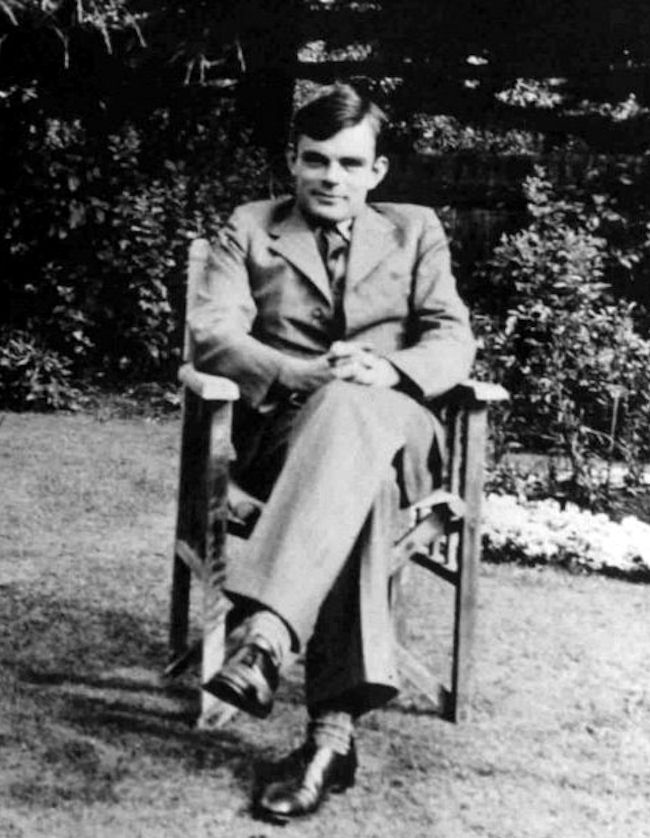
\includegraphics[width=7cm]{images/turing}
    \caption{Hier beschreibt man noch kurz das Bild.
    Ich verwende das mal kurz für Copyright Hinweise:
    This work is in the public domain in its country of origin and other countries and areas where the copyright term is the author's life plus 70 years or less.}
    \label{fig:alan-turing}
    % hier das label, welches oben referenziert wird.
    % man muss die Datei zweimal kompilieren damit die ref richtig angezeigt wird!
    % normalerweise beginnen refs für Abbildungen mit "fig:" und für Tabellen mit "tab:"
\end{figure}

Das ganze geht auch mit tables, diese packt man einfach in eine table float (anstatt figure).

Hier kann jetzt wieder weiter lustiger Text kommen.

\end{document}
